\documentclass[12pt,a4paper,utf8]{ctexart}
\usepackage{ctex,amsmath,amssymb,subfig,cite,graphicx,diagbox,fontspec,fancyhdr,geometry}
\usepackage[ntheorem]{empheq}
\usepackage{enumitem,fullpage,cleveref,cellspace,listings,color,framed}
\definecolor{gray}{rgb}{0.5,0.5,0.5}
\definecolor{dkgreen}{rgb}{.068,.578,.068}
\definecolor{dkpurple}{rgb}{.320,.064,.680}

%set Fortran styles
\lstset{
    frameround=tftf,
    language=Fortran,
    keywords={SELECT,PROGRAM,PRINT,STOP,END,WRITE,INTEGER,REAL,COMPLEX,CHARACTER,LOGICAL,READ,FORMAT,IMPLICIT,PARAMETER,DATA,EQUIVALENCE,TYPE,PAUSE,CONTINUE,CYCLE,EXIT,IF,SELECT,DO,ALLOCATE,DEALLOCATE,WHERE,FORALL,SUBROUTIHNE,CALL,RETURN,FUNCTION,COMMON,BLOCK DATA,SAVE,INTERFACE,CONTAIN,MODULE,USE,PUBLIC,PRIVATE,ENTRY,OPEN,INQUIRE,CLOSE,NAMELIST,POINTER,NULLFY,REWIND,BACKSPACE,ENDFILE
    },
    basicstyle=\small\ttfamily,
    numbers=left,
    numberstyle=\small,
    keywordstyle=\color{blue}\bfseries,
    commentstyle=\color{dkgreen},
    stringstyle=\color{dkpurple},
    backgroundcolor=\color{white},
    tabsize=2,
    showspaces=false,
    showstringspaces=false,
    breaklines=true,
    frame=trBL,
}
\CTEXsetup[format+={\raggedright}]{section}
\setlength{\parindent}{2em}
\geometry{
    textwidth=138mm,
    textheight=215mm,
    left=27mm,
    right=27mm,
    top=25.4mm,
    bottom=25.4mm,
    headheight=2.17cm,
    headsep=4mm,
    footskip=12mm,
    heightrounded,
}
\pagestyle{fancy}
\lhead{\textsl{2021秋-计算物理A}}
\chead{}
\rhead{\textsl{PB19020634-于浩然}}
\lfoot{}
\cfoot{\thepage}
\rfoot{}

\begin{document}
\begin{center}
    {\LARGE\textbf{计算物理作业十五}}\\
    \textrm{于浩然}~~~~~~\textrm{PB19020634}~~~~~~\textrm{2021.12.18}
\end{center}

\section{作业题目}

以$x_{n+1} = \lambda \sin(\pi x_n)$为迭代方程进行迭代:
\begin{enumerate}
    \item[(1)]
        画出系统状态随参数$\lambda$的变化图,要求在图中体现出定值状态、倍周期分叉
        和混沌状态.
    \item[(2)] 列出各个倍周期分叉处的$\lambda$值,求相应的
        \textsl{Feigenbaum}常数.
\end{enumerate}

\section{算法简介}
\subsection{相关概念}

对于如题目所给的以$\lambda$为参数的非线性函数的迭代,随着参数$\lambda$的增大系统
有如下几种状态: 
\begin{itemize}
    \item 绝灭:即$x$最终趋于零.
    \item 定态:系统具有一定值,在图上呈现为一条线.
    \item 倍周期分叉:曲线一分为二,对应着周期为2的解的出现;参数进一步增大时,周期数再次加倍;
        随参数增大分叉出现得越来越快.
    \item 混沌:当参数足够大时,体系进入永不落入定态的涨落态,
        可认为周期为无穷大,轨迹点永不重复.
    \item 周期窗口:在总的混沌范围内出现的具有规律周期的小窗口,这种结构具有无穷嵌套性.
\end{itemize}

\textbf{Feigenbaum常数}用于描述迭代混沌中倍周期分叉的标度行为,其中
\begin{itemize}
    \item $\delta$用于描述横轴方向倍周期分叉的标度行为:

        设第$m$个分叉处$\lambda$值为$\lambda_m$,前后分叉间距的比值趋于一个常数:
        \begin{equation}
            \lim_{m\rightarrow \infty} (\lambda_m -
            \lambda_{m-1})/(\lambda_{m+1}/\lambda_m) = \delta
            = 4.669201
        \end{equation}

    \item $\alpha$用于描述纵轴方向倍周期分叉的标度行为:

        在图上作$x_n=1/2$的直线与放大的分叉曲线相交,
        设在第$m$个分叉处纵向间距为$d_m$,则
        \begin{equation}
            \lim_{m\rightarrow \infty} d_m/d_{m+1} = \alpha = 2.502908
        \end{equation}
\end{itemize}

\subsection{具体方法}

对于足够密集取的$\lambda$值,由给定初值$x_0$计算迭代$N-m,N-m+1,\cdots,N$
次的结果$x_n$,以$\lambda$为
横轴,以$x_n$为纵轴,画出散点图,恰当取参数便能体现定值、倍周期分叉和混沌状态.

得到图像后容易找出各分叉点处的$\lambda$值,由此可以计算Feigenbaum常数值.
\section{编程实现}

使用FORTRAN90进行编程,通过简单的函数迭代得到迭代结果$x_n$和对应$\lambda$值的数组.
不妨取$\lambda$步进值$ \mathtt{step}=0.00001$,共取$\mathtt{lnum}=100000$个,
即$\lambda \in [0,1]$;对每个$\lambda$值迭代$\mathtt{ites}=10000$次,
并取最后的$\mathtt{counts}=30$个数记录至文件并随后绘图.

由于能够辨认的分叉数极其有限,只需辨认并考虑图中前几个分叉处的坐标值,并可由此直接
计算相应的Feigenbaum常数.
\section{计算结果}
\subsection{系统状态随参数$\lambda$变化图}

$\lambda\in [0,5]$的图像总体如下,显然从图中可看到2.1中所讲的各种状态:
\begin{figure}[!h]
    \centering
    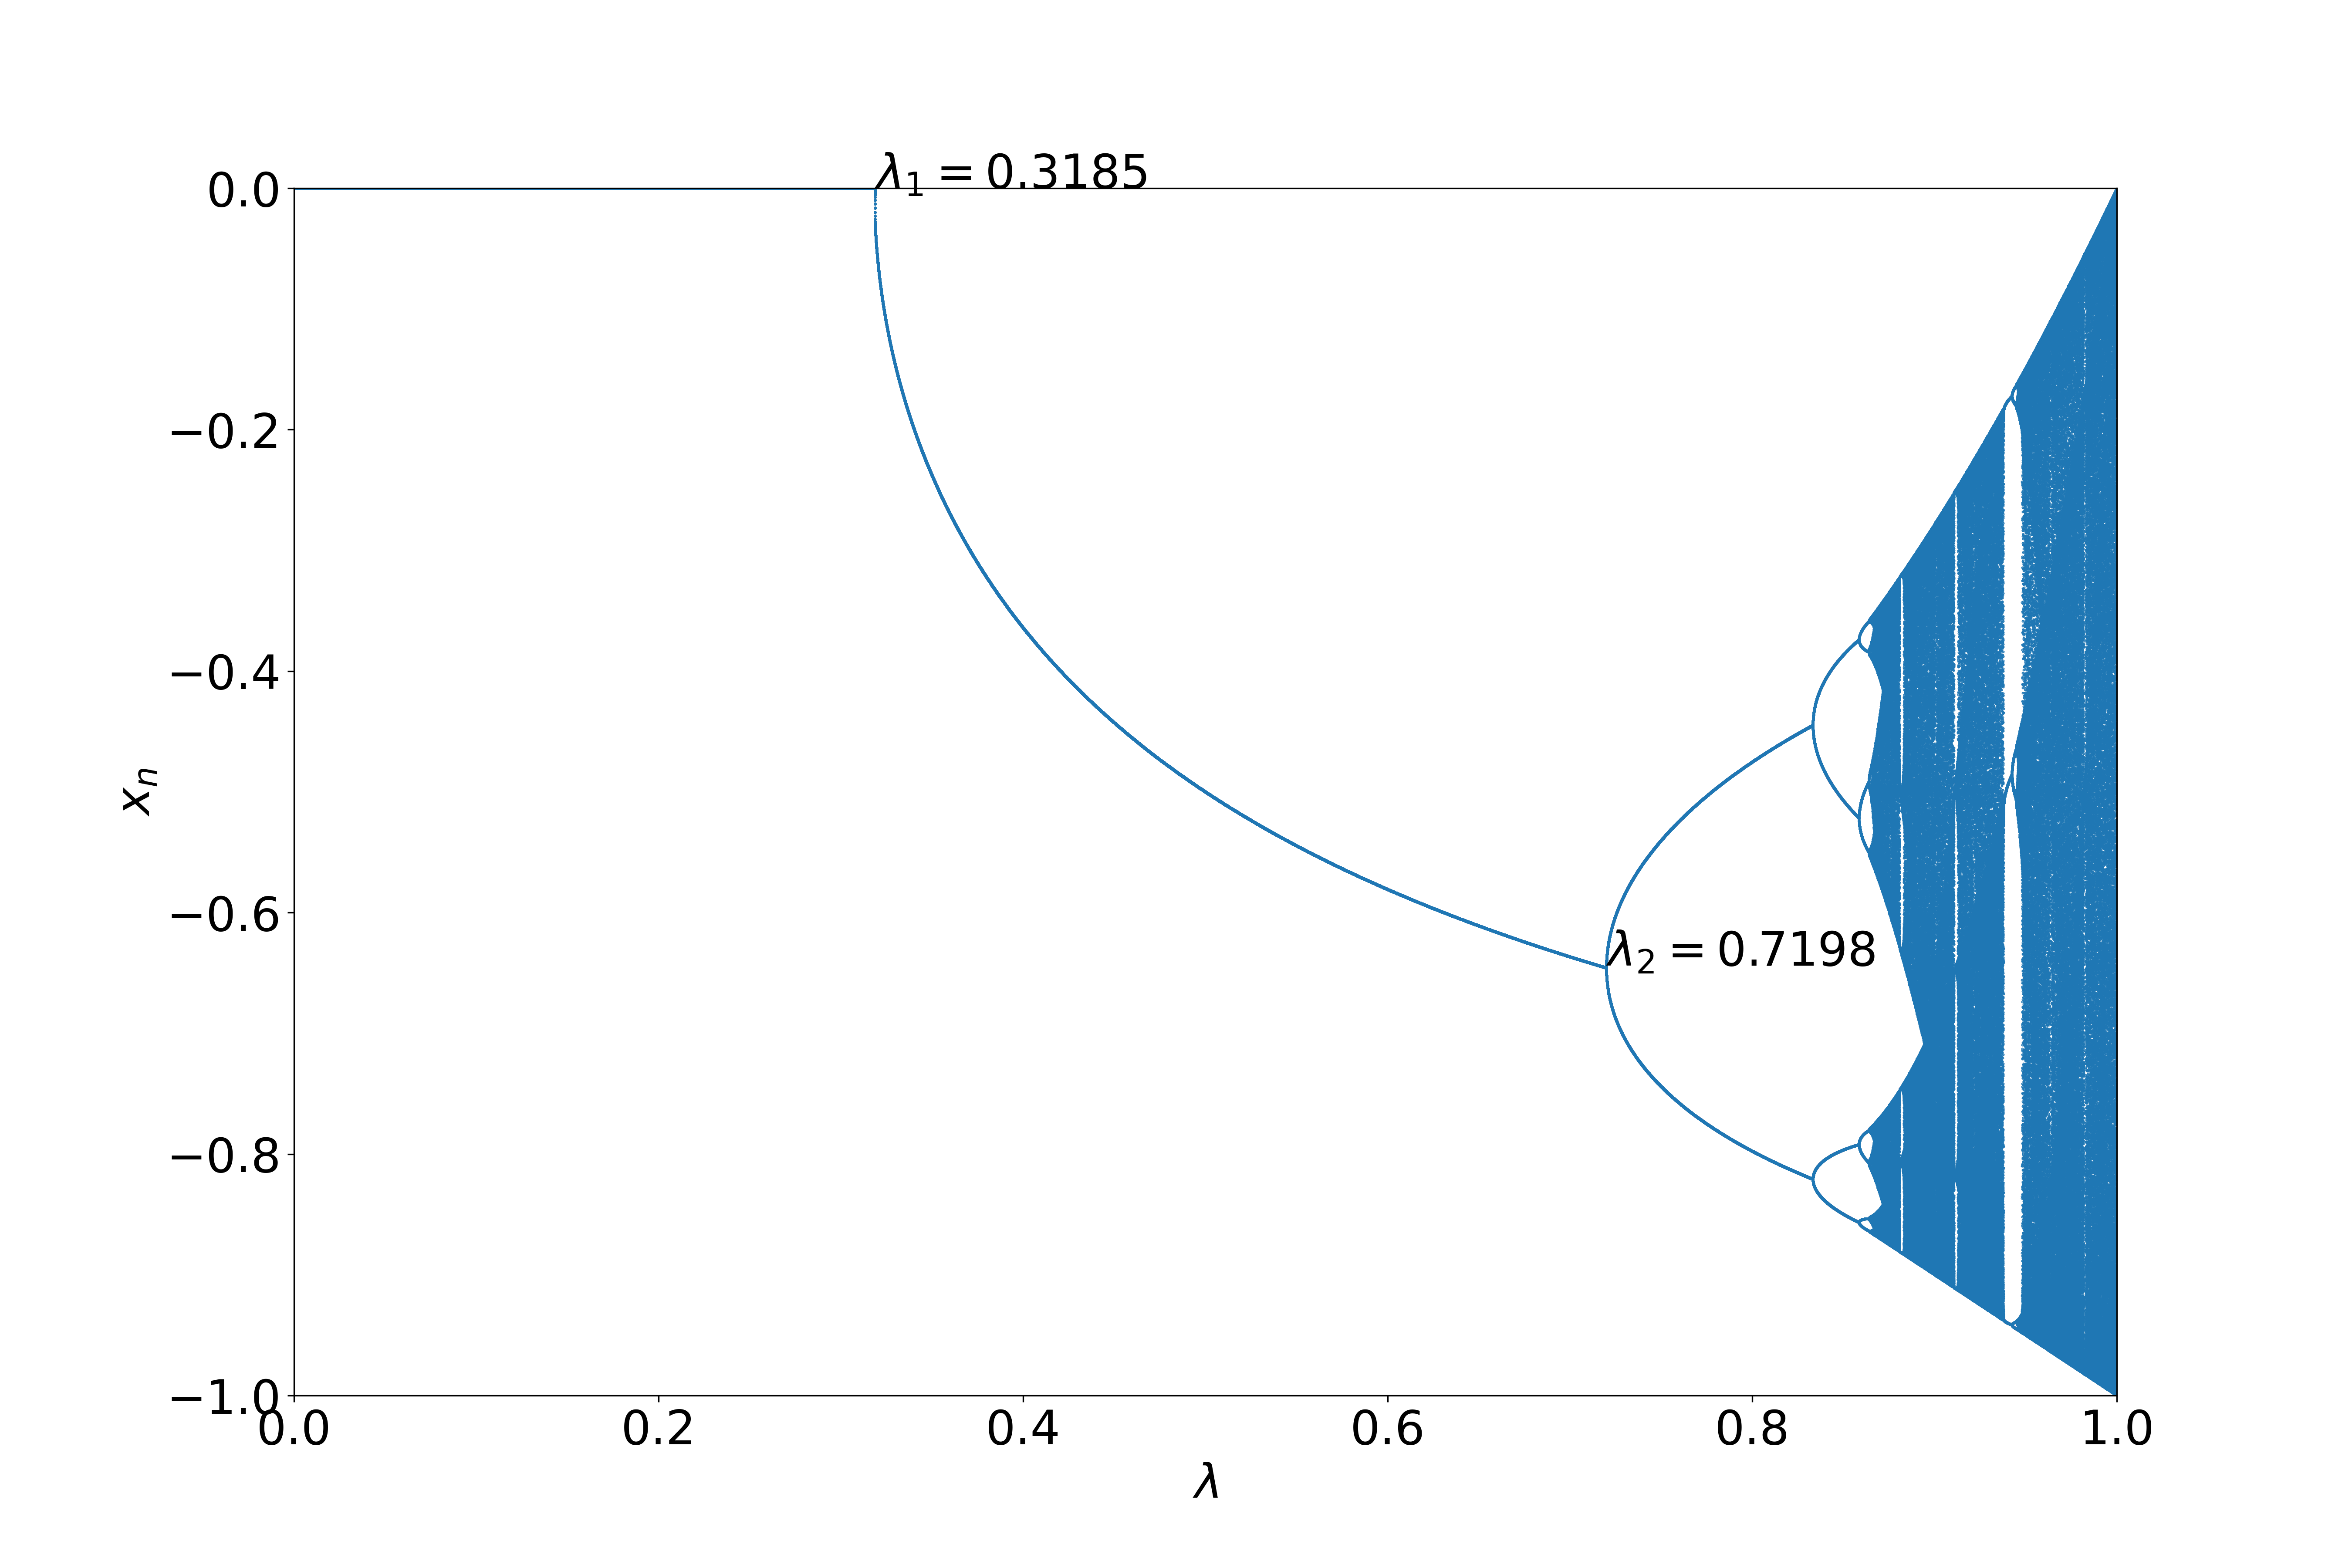
\includegraphics[width=0.8\textwidth]{half.png}
    \caption{系统状态随$\lambda$变化图}
\end{figure}
\begin{itemize}
    \item 当$\lambda \in(0,0.318)$时,系统处于绝灭态,迭代结果均为零;
    \item 当$\lambda \in(0.318,
        0.720)$时,系统处于定态,这时迭代最终趋于一个不为零的唯一结果;
    \item 当$\lambda \in (0.720, 0.870)$时,
        系统进入了倍周期分叉,分叉速度越来越快,最终到达混沌;
    \item 当$\lambda > 0.870$时,系统进入混沌,这时仍能看到规律性的周期窗口.
\end{itemize}

\subsection{图像缩放并寻找分叉点}

我们从上面图中通过缩放已经将前两个分叉点的坐标确定到小数点后四位,还要进一步
确定其他的分叉点,为了直观不妨取图二中$\lambda \in(0.82,
0.88), x_n\in(-0.9, -0.3)$区域进行缩放,再选取$\lambda \in (0.857, 0.866), x_n \in (-0.58,
-0.35)$区域,读取$\lambda_m$值如下图:
\begin{figure}[!h]
    \centering
    \subfloat[$\lambda \in (0.82,0.88)$]{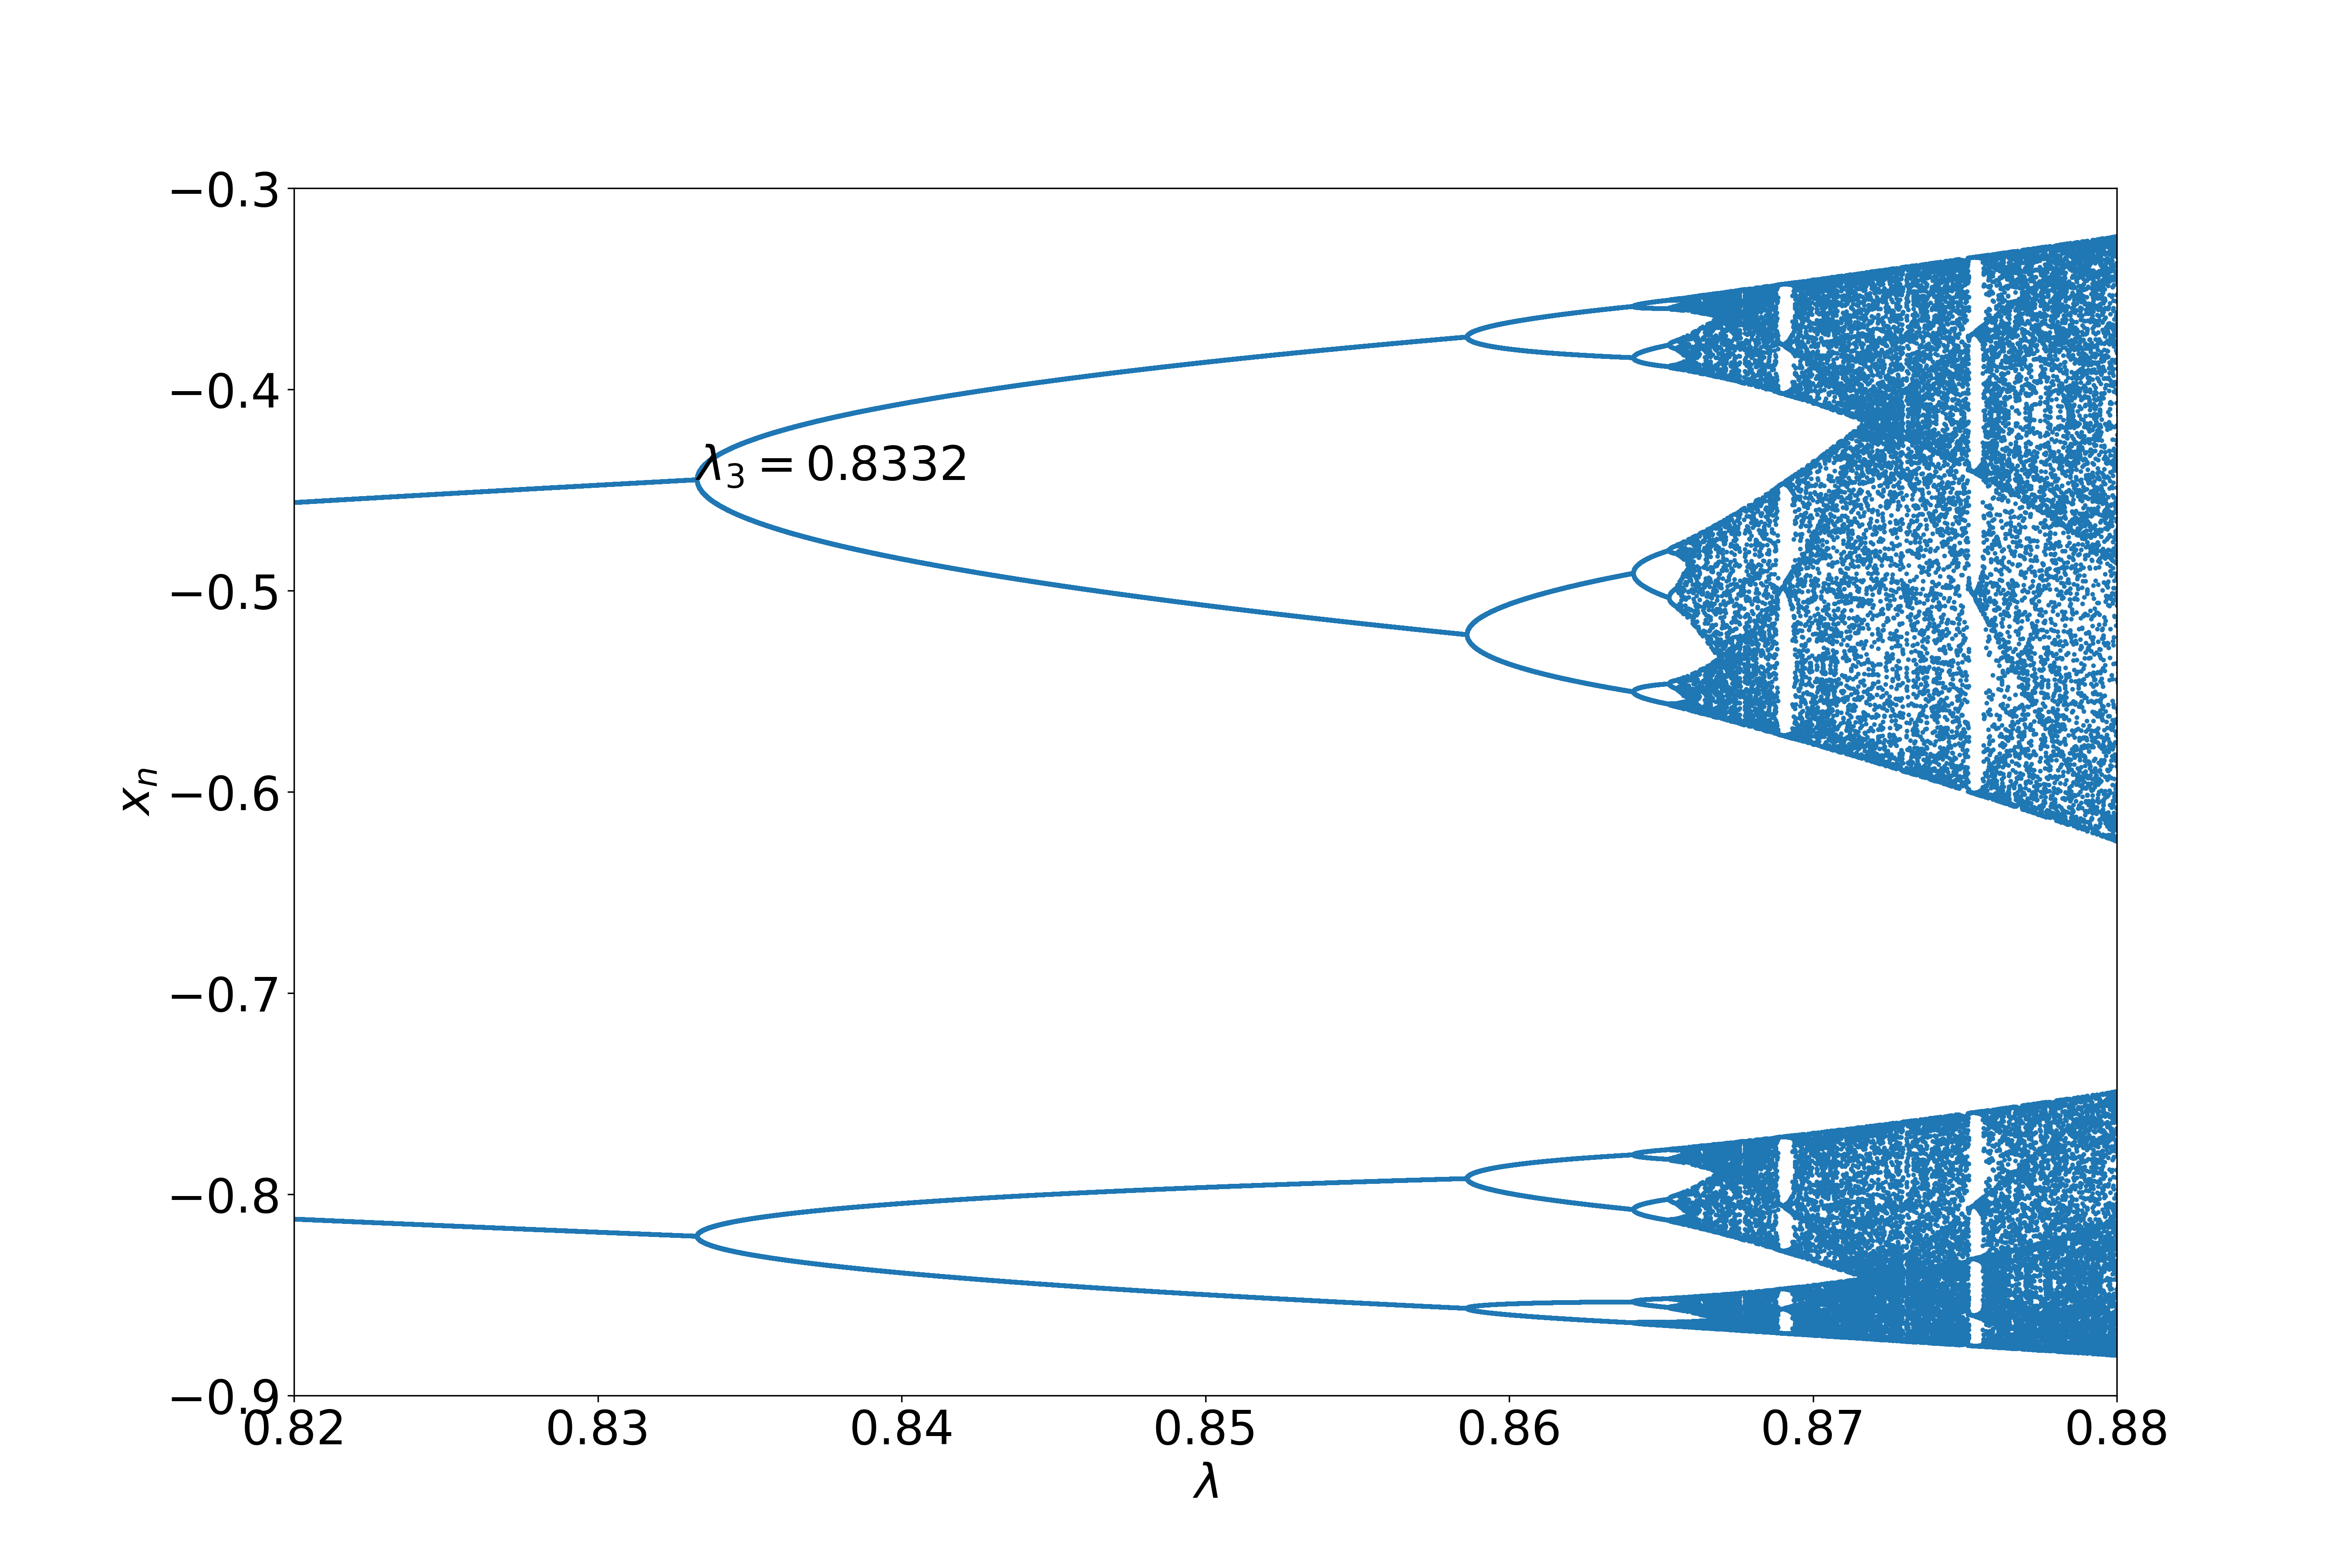
\includegraphics[width=0.5\textwidth]{qua.png}}
    \hfill
    \subfloat[$\lambda \in (0.857, 0.866)$]{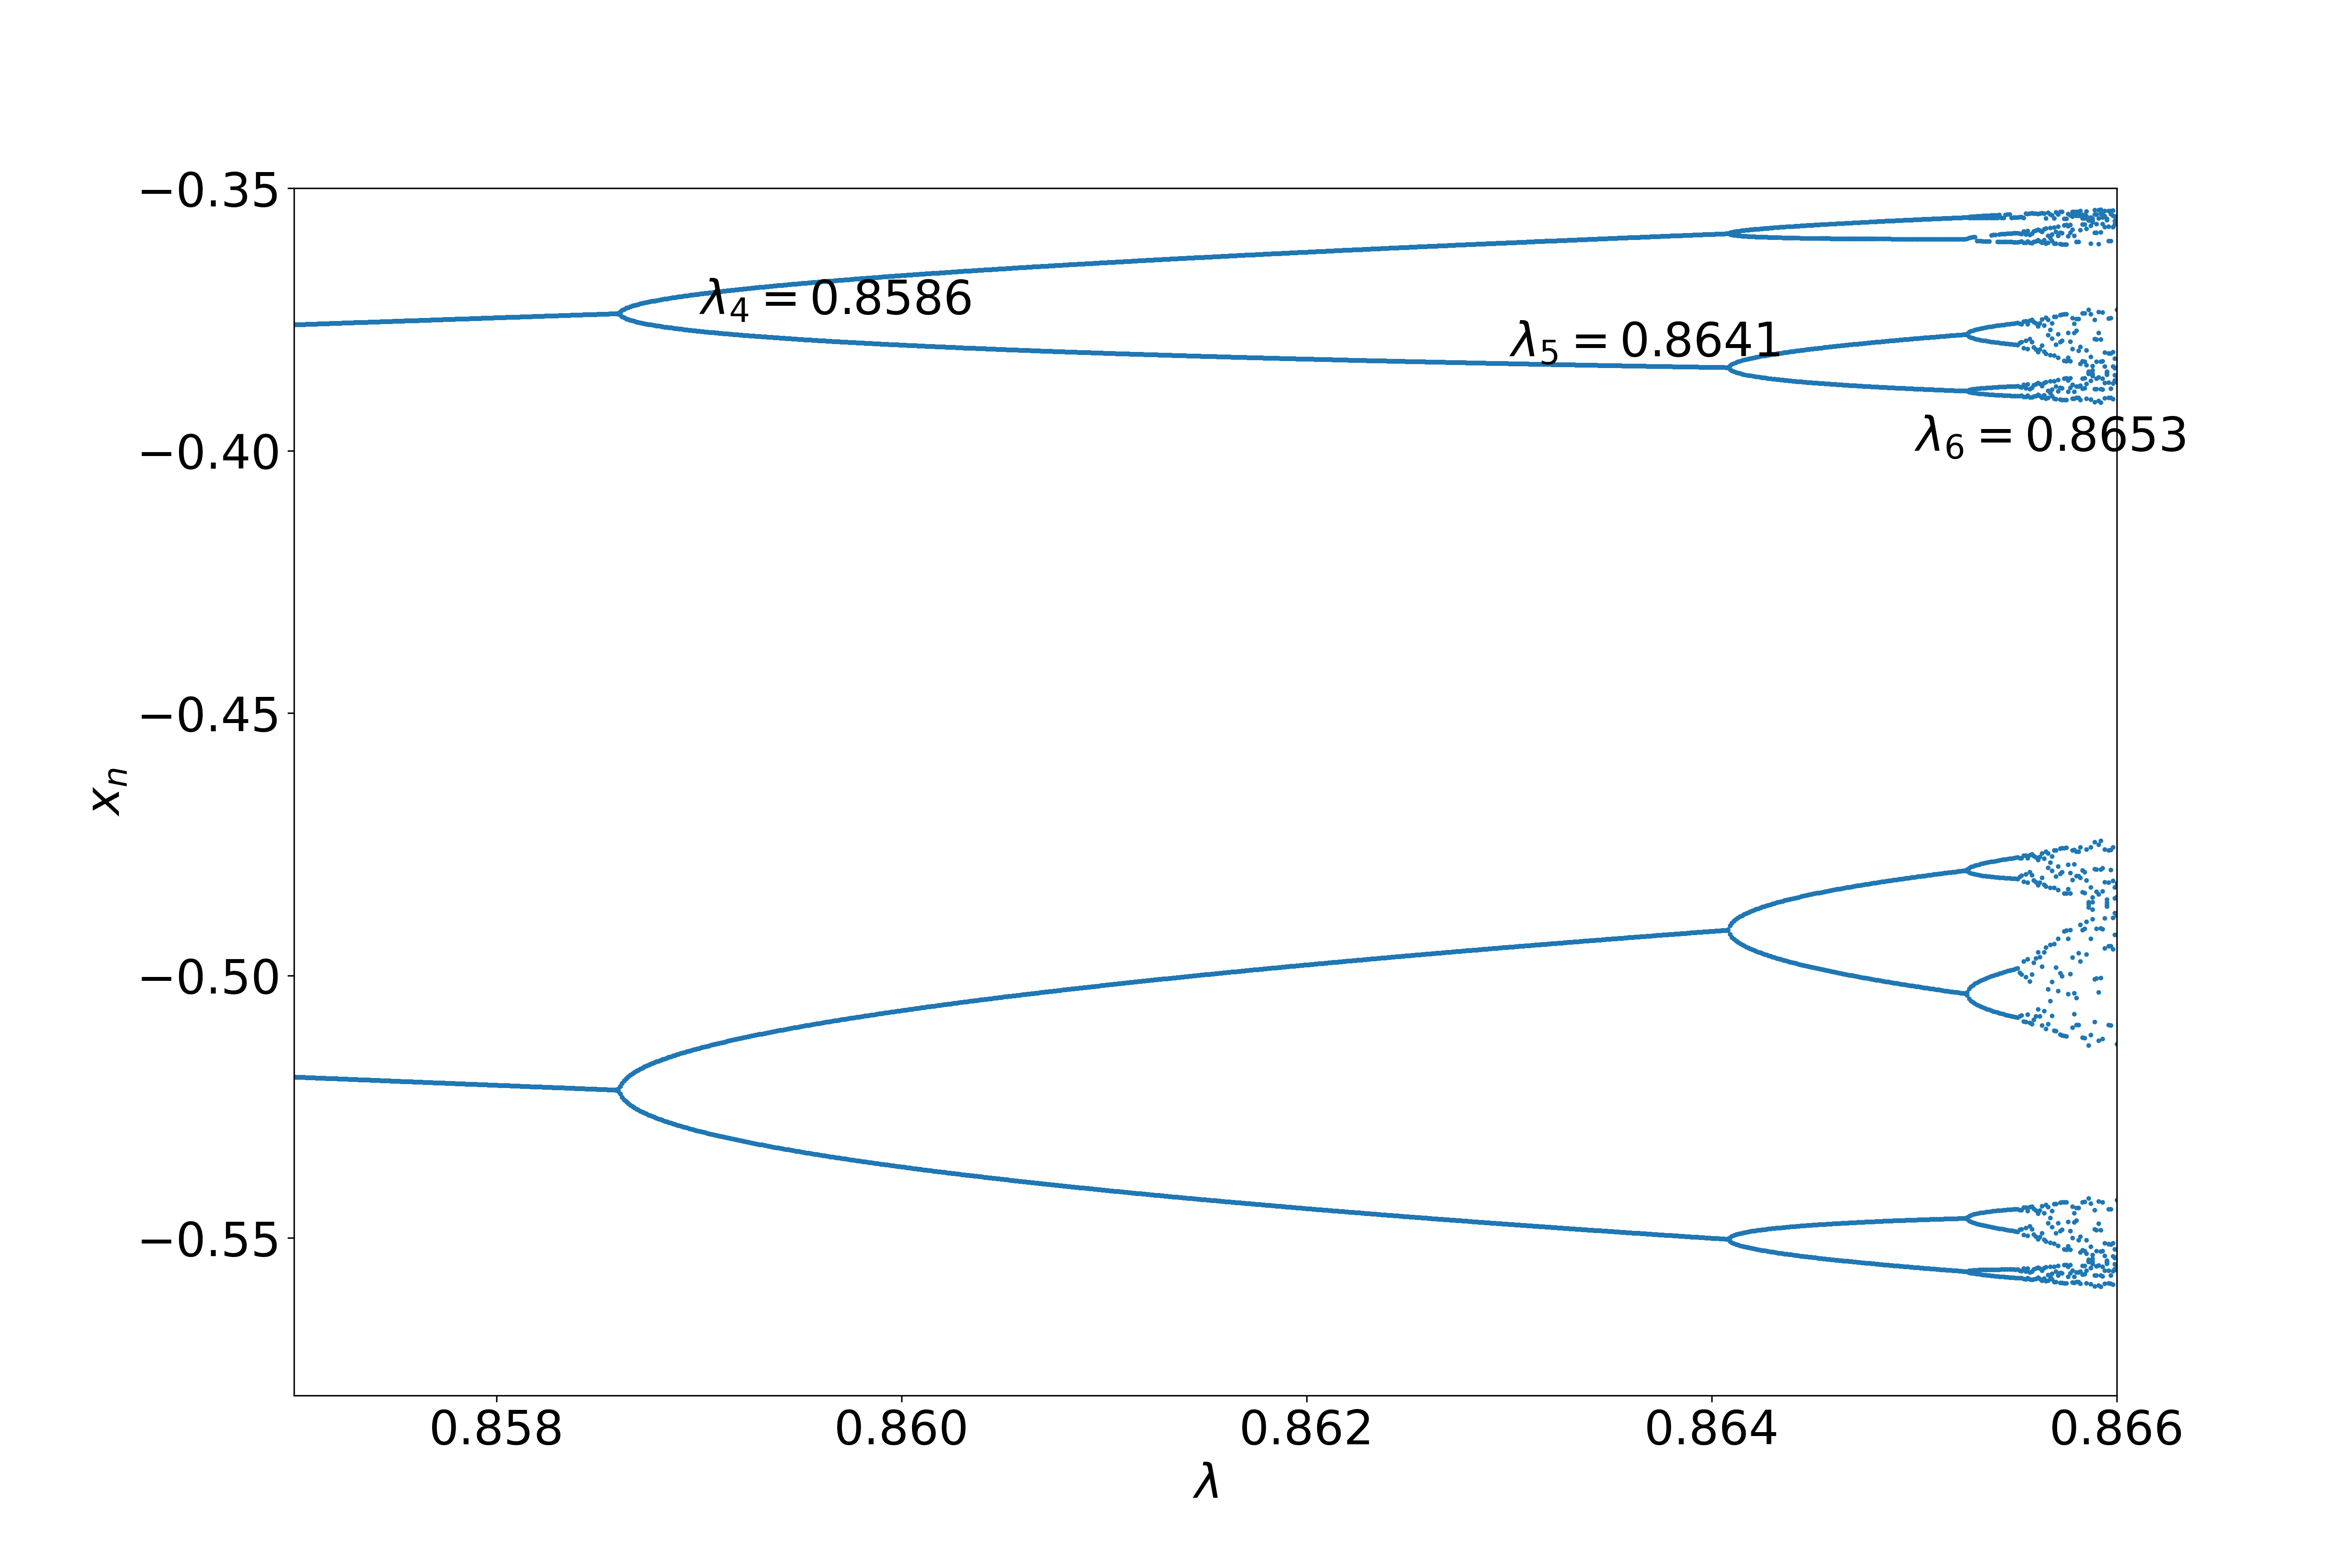
\includegraphics[width=0.5\textwidth]{oct.png}}
    \caption{系统状态随$\lambda$变化图}
\end{figure}

根据这些点即可计算Feigenbaum常数.

\newpage
\subsection{Feigenbaum常数计算}

将各分叉处$\lambda$值列表如下:
\begin{table}[!h]
\centering
\caption{$\lambda_m$值与计算所得$\delta$值表}
\begin{tabular}{|l|l|l|l|l|l|l|}
\hline
$m$                                                   & 1      & 2      & 3      & 4      & 5      & 6      \\ \hline
$\lambda_m$                                           & 0.3185 & 0.7198 & 0.8332 & 0.8586 & 0.8641 & 0.8653 \\ \hline
$\lambda_m-\lambda_{m-1}$                             &        & 0.4013 & 0.1134 & 0.0254 & 0.0055 & 0.0012 \\ \hline
$(\lambda_m-\lambda_{m-1})/(\lambda_{m+1}-\lambda_m)$ &        & 3.539  & 4.465  & 4.618  & 4.583  &        \\ \hline
\end{tabular}
\end{table}

与$\delta$理论值比较图如下:
\begin{figure}[!h]
    \centering
    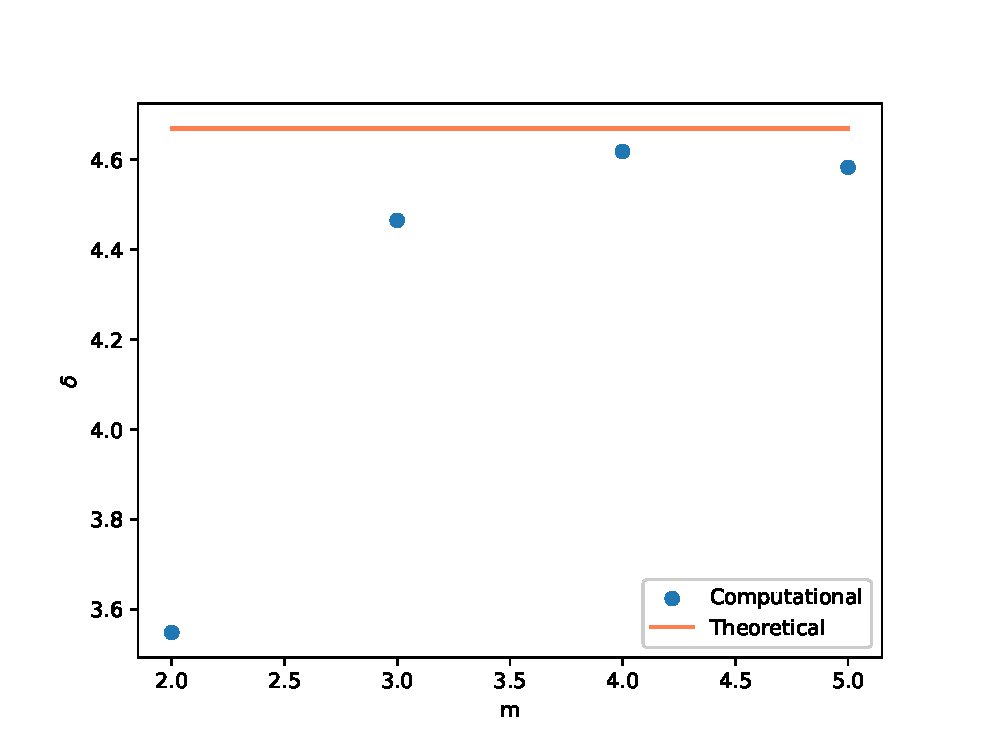
\includegraphics[width=0.6\textwidth]{err1.eps}
    \caption{$\delta$计算值情况}
\end{figure}
由图可得,除第一个点外计算结果较好. 

在图1基础上作$x_n=1/2$直线,与曲线相交如下图:
\begin{figure}[!h]
    \centering
    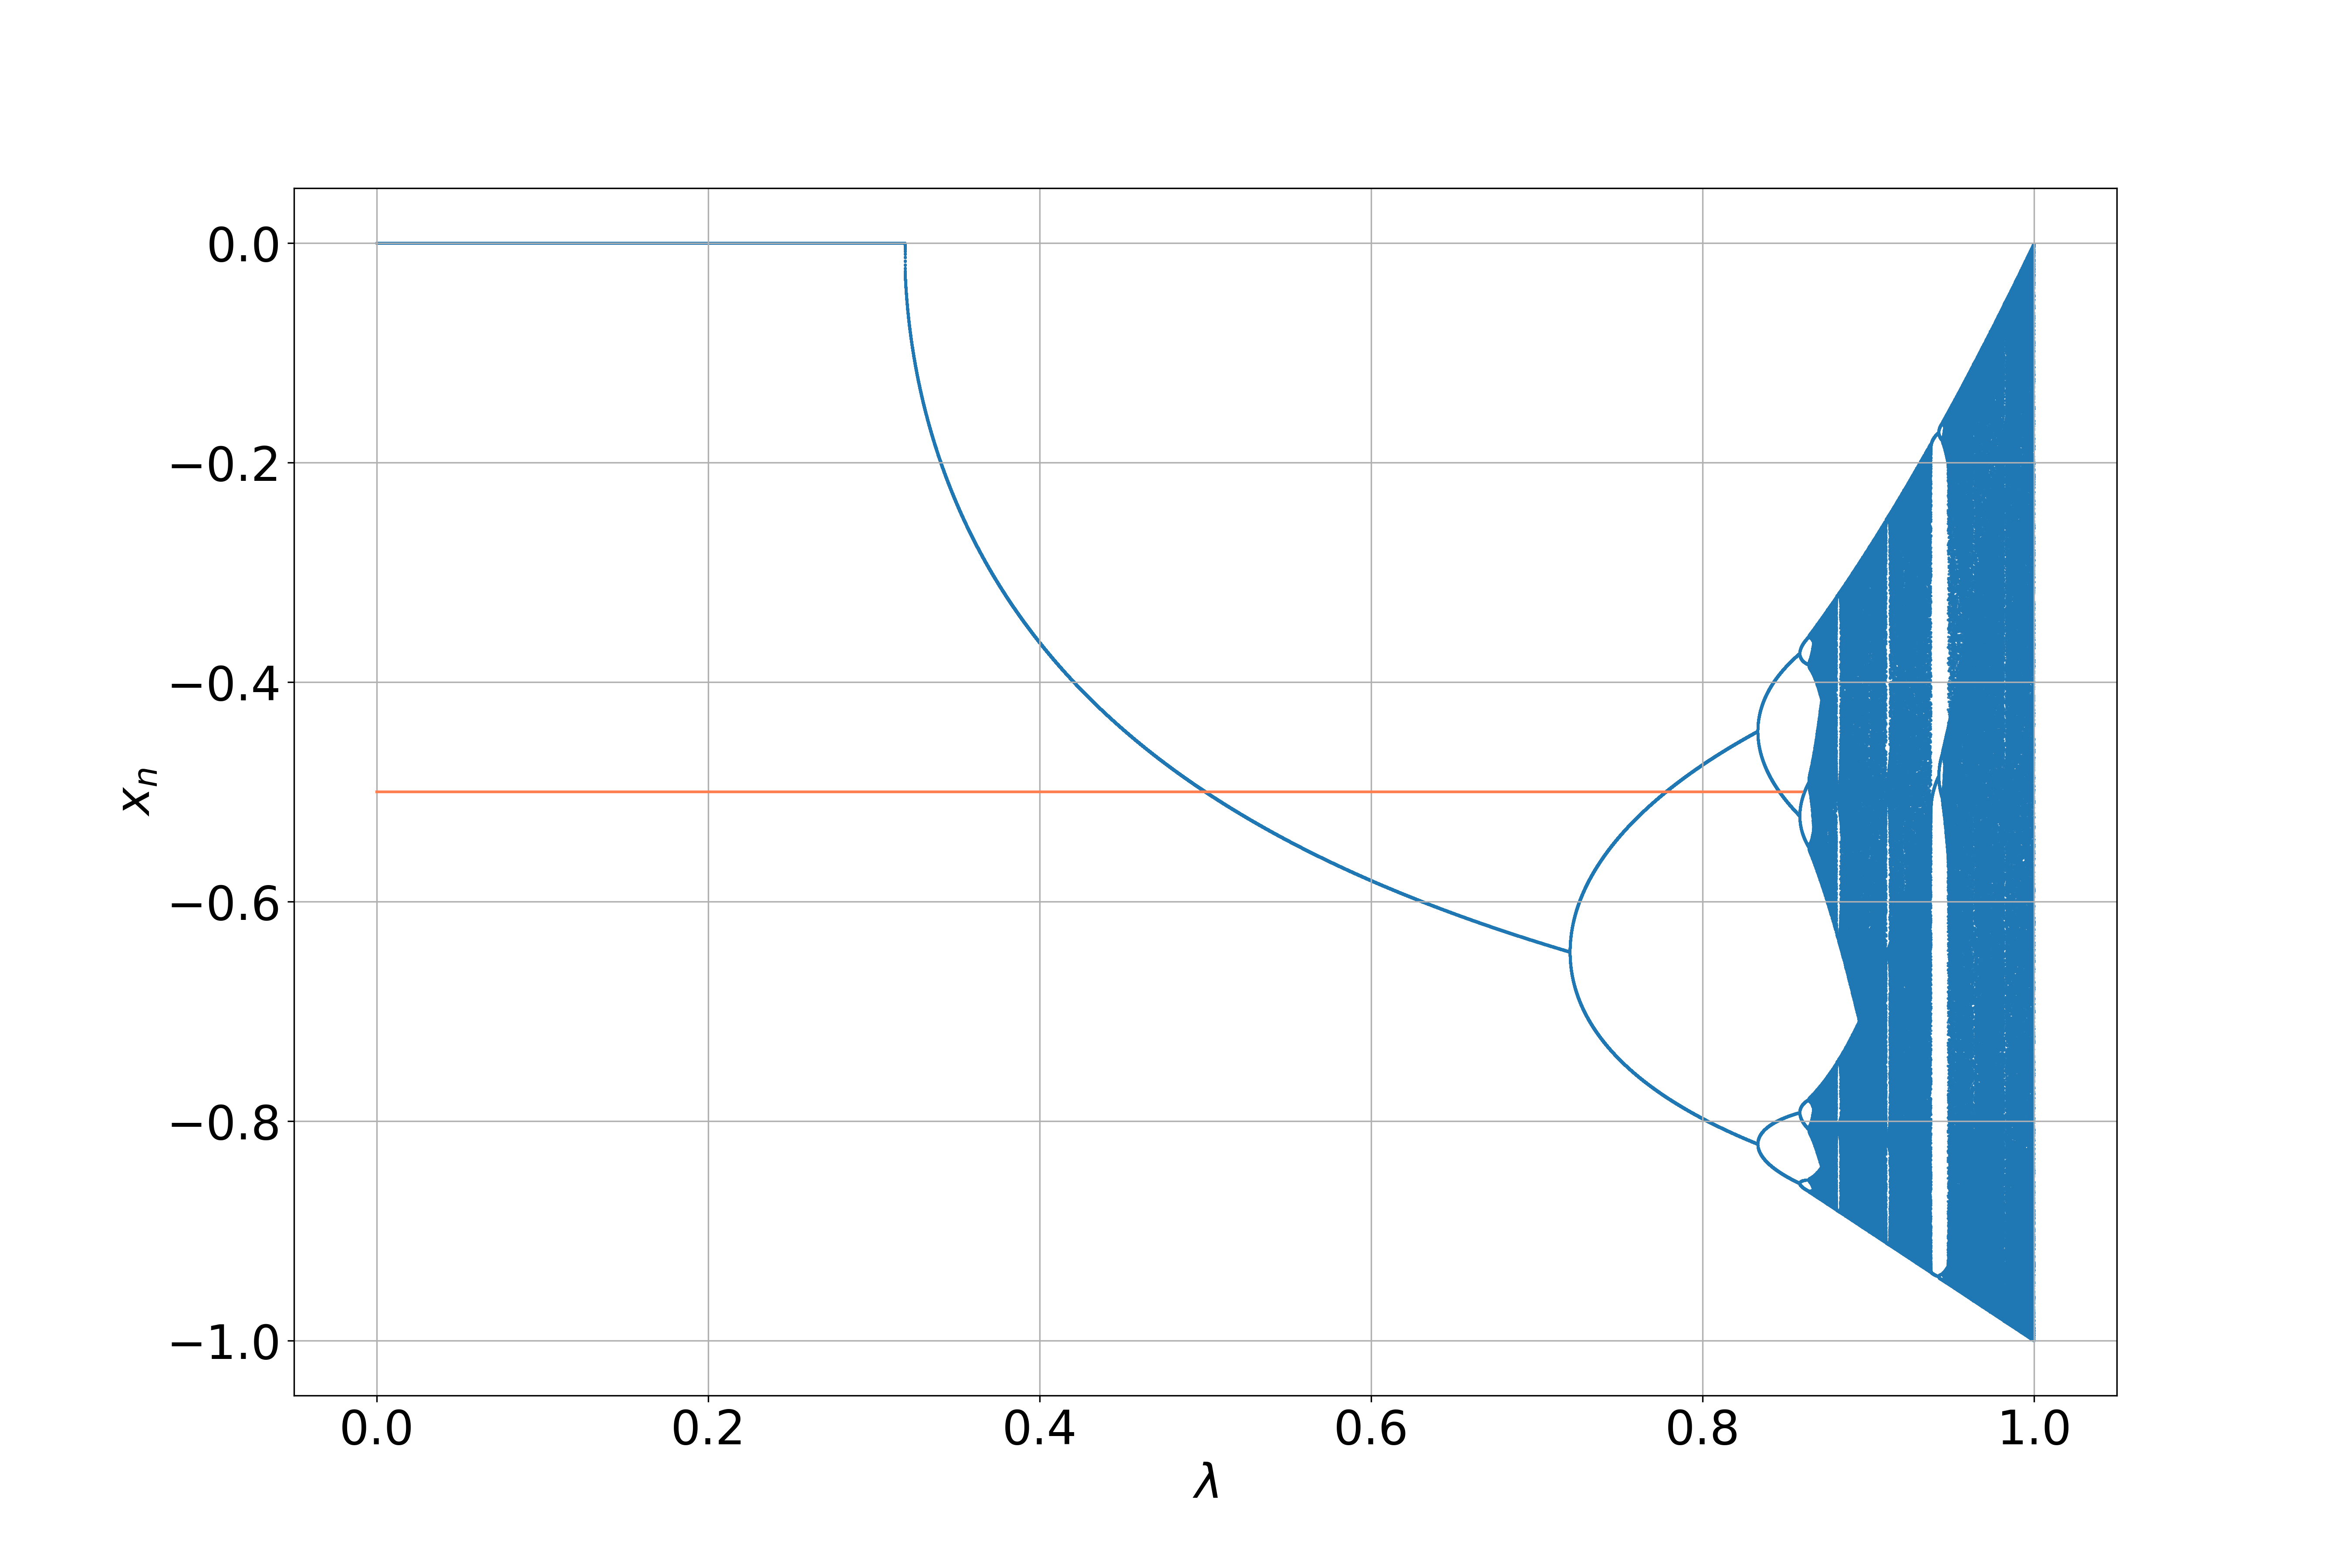
\includegraphics[width=0.6\textwidth]{alpha.png}
    \caption{$x_n=1/2$与曲线相交图}
\end{figure}

从图中读取交点并读取$d_m$
计算$\alpha$值列表如下:
\begin{table}[!h]
    \centering
    \caption{计算所得$\alpha$值表}
\begin{tabular}{|l|l|l|l|l|l|l|}
\hline
$m$           & 3      & 4      & 5      & 6      \\ \hline
$d_m$         & 0.2777 & 0.1073 & 0.0425 & 0.0170 \\ \hline
$d_m/d_{m+1}$ & 2.588  & 2.525  & 2.5000 &        \\ \hline
\end{tabular}
\end{table}

与理论值比较如下图:
\begin{figure}[!h]
    \centering
    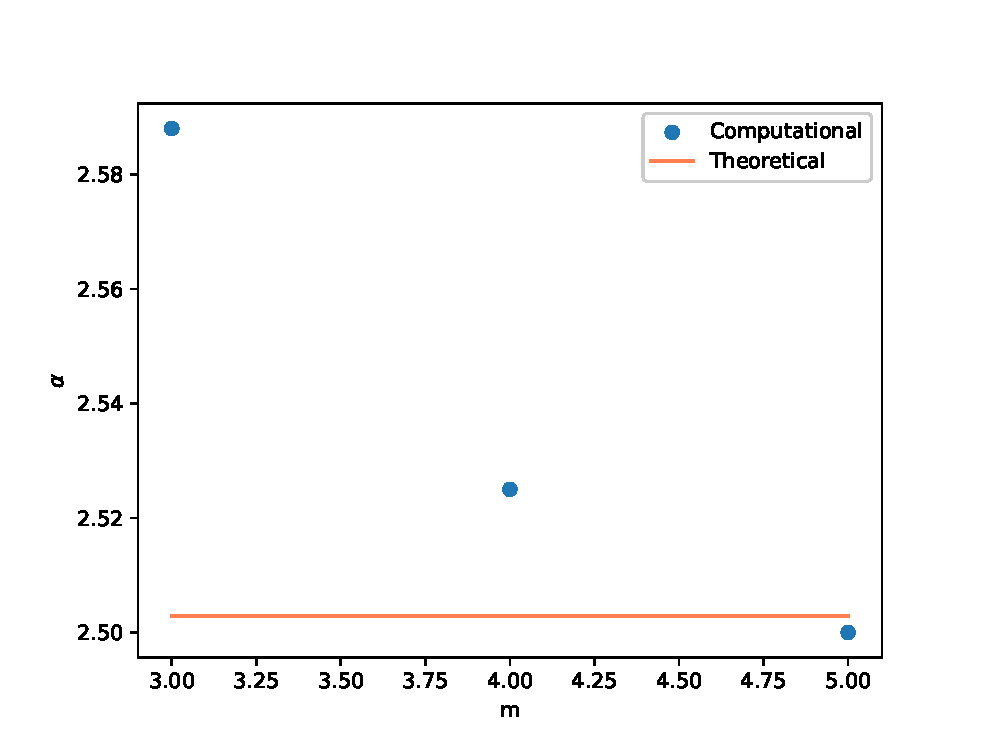
\includegraphics[width=0.8\textwidth]{err2.eps}
    \caption{$\alpha$计算值情况}
\end{figure}

可见计算的精度不高,也算能够接受.
\section{结论}

本题中模拟了迭代函数体系的混沌状态,通过直观的图像加深了对其的理解.
计算的精度受到 \texttt{step}取值的约束(本题中 \texttt{step}=0.00001),在加上读取数据造成的误差,
导致计算的精度不够高. 此外,对于这种分形的结构,计算机的浮点运算在缩放的区域内
误差将会不可控制,同样需要考虑.

\section{源代码}

Fortran90代码如下:
\begin{framed}
\begin{lstlisting}[language=Fortran]
MODULE CHAO
IMPLICIT NONE
REAL(KIND=8) :: pi = 3.1415927
CONTAINS
REAL(KIND=8) FUNCTION y(lambda, x)
    REAL(KIND=8), INTENT(IN) :: lambda, x
    y = lambda * SIN(pi * x)
END FUNCTION y
SUBROUTINE Iteration(step, ites, lnum, counts, filename)
    REAL(KIND=8), INTENT(IN) :: step
    INTEGER(KIND=4), INTENT(IN) :: lnum, ites, counts
    CHARACTER(LEN=*), INTENT(IN) :: filename
    REAL(KIND=8) :: lambda, x, sol(lnum*counts, 2)
    INTEGER(KIND=4) :: i, j
    lambda = 0
    DO i = 1, lnum
        x = 1
        DO j = 1, ites - counts
            x = y(lambda, x)
        END DO
        DO j = 1, counts
            x = y(lambda, x)
            sol((i-1)*counts + j, 1) = lambda
            sol((i-1)*counts + j, 2) = x
        END DO
        lambda = lambda + step
    END DO
    OPEN (1, file=filename)
    WRITE (1, *) sol
    CLOSE (1)
END SUBROUTINE Iteration
END MODULE CHAO

PROGRAM MAIN
    USE CHAO    
    IMPLICIT NONE    
    CALL Iteration(0.00001_8, 10000, 100000, 30, 'sol.dat')
END PROGRAM MAIN
\end{lstlisting}
\end{framed}
\end{document}

